\documentclass[11pt]{article}

% ---------- Packages (per course conventions) ----------
\usepackage[margin=1in]{geometry}
\usepackage{graphicx}
\usepackage{float}
\usepackage{booktabs}
\usepackage{siunitx}
\usepackage{amsmath}
\usepackage{amssymb}
\usepackage{tikz}
\usetikzlibrary{arrows.meta,calc,patterns,decorations.pathmorphing}
\usepackage{tcolorbox}
\usepackage{enumitem}
\usepackage{xcolor}
\usepackage{hyperref}
\hypersetup{colorlinks=true, linkcolor=black, urlcolor=blue}

\setlength{\parindent}{0pt}
\setlength{\parskip}{0.6\baselineskip}

\newcommand{\assignmentNumber}{6}
\newcommand{\assignedDate}{23 Oct 2026}
\newcommand{\dueDate}{2 Nov 2026}

\newtcolorbox{finalanswer}{
    colback=white, colframe=black, boxrule=1pt,
    title=Answer, fonttitle=\bfseries, coltitle=black,
    colbacktitle=white
}

\tikzset{
  force/.style={-{Stealth[length=2.6mm]}, very thick, red!75!black},
  mem/.style={line width=3pt, blue!45!gray},
  load/.style={thin, blue!60!black},
  loadarrow/.style={-{Stealth[length=1.4mm]}, thin, blue!60!black},
  dim/.style={{Stealth[length=1.6mm]}-{Stealth[length=1.6mm]}, thin, gray},
  axis/.style={-{Stealth[length=2mm]}, thin},
  every node/.style={font=\small}
}
\newcommand{\pin}[1]{\fill[white] (#1) circle (2.2pt); \draw (#1) circle (2.2pt);}
\newcommand{\axes}[1]{\draw[axis] #1 -- ++(0.8,0) node[right]{$x$}; \draw[axis] #1 -- ++(0,0.8) node[above]{$y$};}

\newcommand{\problemhead}[2]{%
    \clearpage
    \section*{Problem #1}
    \textbf{Given / Find:} #2
}

\begin{document}

% =========================================================
% COVERSHEET
% =========================================================
\begin{titlepage}
    \centering
    \vspace*{2cm}
    {\LARGE \bfseries ENGR 225: Mechanics 1} \\[0.3cm]
    {\Large Homework Coversheet} \\[0.3cm]
    {\large Assoc.\ Prof.\ Clayton Byers} \\[2cm]

    \begin{flushleft}
        \Large
        \textbf{NAME:} \underline{\makebox[10cm][l]{Sean Balbale}} \\[1cm]
        \textbf{DATE:} \underline{\hspace{10cm}} \\[1cm]
        \textbf{ASSIGNMENT:} \underline{\makebox[9cm][l]{Homework 6}} \\[2cm]
    \end{flushleft}

    \large
    \textbf{Level of involvement of AI, LLMs, or related tools in the completion of this assignment:}

    \vspace{1cm}

    \begin{flushleft}
        \Large
        $\square$ \quad None \\[0.7cm]
        $\blacksquare$ \quad Minor \\[0.7cm]
        $\square$ \quad Major \\[0.7cm]
        $\square$ \quad Extensive \\[1.5cm]
    \end{flushleft}

    \normalsize
    \textit{Mark the box that applies (e.g., replace $\square$ with $\blacksquare$, or type an X beside it, before compiling/printing). Your disclosure does not affect your grade -- it keeps you accountable for the work you are doing.}
\end{titlepage}

% \section*{ENGR 225 -- Homework \assignmentNumber}
% \textbf{Assigned:} \assignedDate \hfill \textbf{Due:} \dueDate

% Sign convention throughout: $+x$ right, $+y$ up, CCW moments positive. A negative result means the force acts opposite to the direction drawn on the FBD.

% =========================================================
% PROBLEM 1
% =========================================================
\problemhead{1}{A \SI{100}{lb} block hangs from three pulley systems. Pulleys and cords are massless and frictionless, so tension is constant along any one cord. Find the pull $P$ for equilibrium in each.}

\textbf{Sketch:} FBDs of the movable pulleys, cut just above them.

\begin{center}
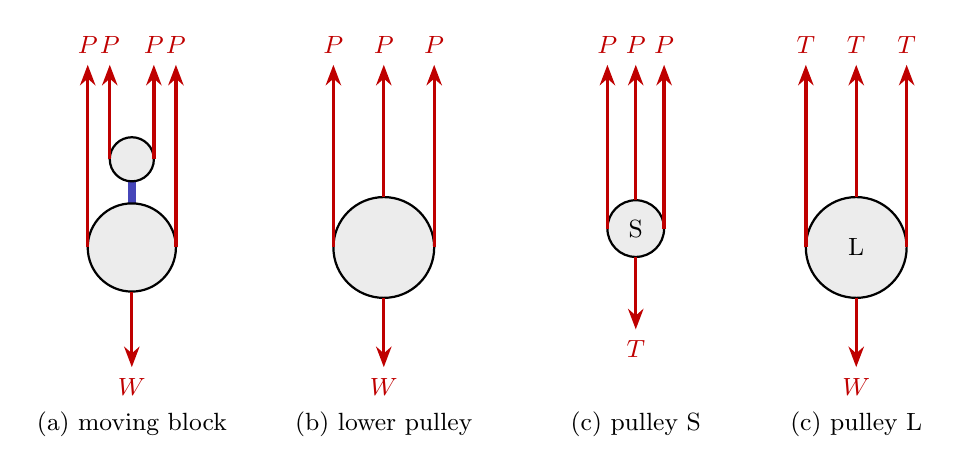
\begin{tikzpicture}[scale=0.8]
% (a) moving block: small pulley over large pulley
\begin{scope}
  \draw[mem] (0,0) -- (0,1.4);
  \draw[thick,fill=gray!15] (0,1.4) circle (0.35);
  \draw[thick,fill=gray!15] (0,0) circle (0.7);
  \draw[force] (-0.35,1.4) -- (-0.35,2.9) node[above]{$P$};
  \draw[force] (0.35,1.4) -- (0.35,2.9) node[above]{$P$};
  \draw[force] (-0.7,0) -- (-0.7,2.9) node[above]{$P$};
  \draw[force] (0.7,0) -- (0.7,2.9) node[above]{$P$};
  \draw[force] (0,-0.7) -- (0,-1.9) node[below]{$W$};
  \node at (0,-2.8) {(a) moving block};
\end{scope}
% (b)
\begin{scope}[xshift=4cm]
  \draw[thick,fill=gray!15] (0,0) circle (0.8);
  \draw[force] (-0.8,0) -- (-0.8,2.9) node[above]{$P$};
  \draw[force] (0,0.8) -- (0,2.9) node[above]{$P$};
  \draw[force] (0.8,0) -- (0.8,2.9) node[above]{$P$};
  \draw[force] (0,-0.8) -- (0,-1.9) node[below]{$W$};
  \node at (0,-2.8) {(b) lower pulley};
\end{scope}
% (c) small movable pulley S
\begin{scope}[xshift=8cm,yshift=0.3cm]
  \draw[thick,fill=gray!15] (0,0) circle (0.45); \node at (0,0) {S};
  \draw[force] (-0.45,0) -- (-0.45,2.6) node[above]{$P$};
  \draw[force] (0,0.45) -- (0,2.6) node[above]{$P$};
  \draw[force] (0.45,0) -- (0.45,2.6) node[above]{$P$};
  \draw[force] (0,-0.45) -- (0,-1.6) node[below]{$T$};
  \node at (0,-3.1) {(c) pulley S};
\end{scope}
% (c) large pulley L
\begin{scope}[xshift=11.5cm]
  \draw[thick,fill=gray!15] (0,0) circle (0.8); \node at (0,0) {L};
  \draw[force] (-0.8,0) -- (-0.8,2.9) node[above]{$T$};
  \draw[force] (0,0.8) -- (0,2.9) node[above]{$T$};
  \draw[force] (0.8,0) -- (0.8,2.9) node[above]{$T$};
  \draw[force] (0,-0.8) -- (0,-1.9) node[below]{$W$};
  \node at (0,-2.8) {(c) pulley L};
\end{scope}
\end{tikzpicture}
\end{center}

\textbf{Solution:}

\textbf{(a)} Four cord segments support the block:
\[
\textstyle\sum F_y = 4P - W = 0 \;\Rightarrow\; P = \frac{\SI{100}{lb}}{4} = \SI{25.0}{lb}
\]

\textbf{(b)} Three cord segments support the lower pulley:
\[
\textstyle\sum F_y = 3P - W = 0 \;\Rightarrow\; P = \frac{\SI{100}{lb}}{3} = \SI{33.3}{lb}
\]

\textbf{(c)} Three $P$ segments hold S; three $T$ segments hold L.
\begin{align*}
\text{S:}\quad \textstyle\sum F_y &= 3P - T = 0 \;\Rightarrow\; T = 3P\\
\text{L:}\quad \textstyle\sum F_y &= 3T - W = 9P - W = 0 \;\Rightarrow\; P = \frac{\SI{100}{lb}}{9} = \SI{11.1}{lb}
\end{align*}

\begin{finalanswer}
(a) $P = \SI{25.0}{lb}$ \qquad (b) $P = \SI{33.3}{lb}$ \qquad (c) $P = \SI{11.1}{lb}$
\end{finalanswer}

% =========================================================
% PROBLEM 2
% =========================================================
\problemhead{2}{$AC$ is fixed at $A$ and carries a triangular load peaking at \SI{500}{lb/ft} at mid-span. Link $CD$ rises \SI{6}{ft} over \SI{8}{ft}. $DB$ (\SI{9}{ft}) carries \SI{700}{lb/ft} at $D$ tapering to zero at the pin $B$. Find $A_x$, $A_y$, $M_A$, $B_x$, $B_y$.}

\textbf{Sketch:}

\begin{center}
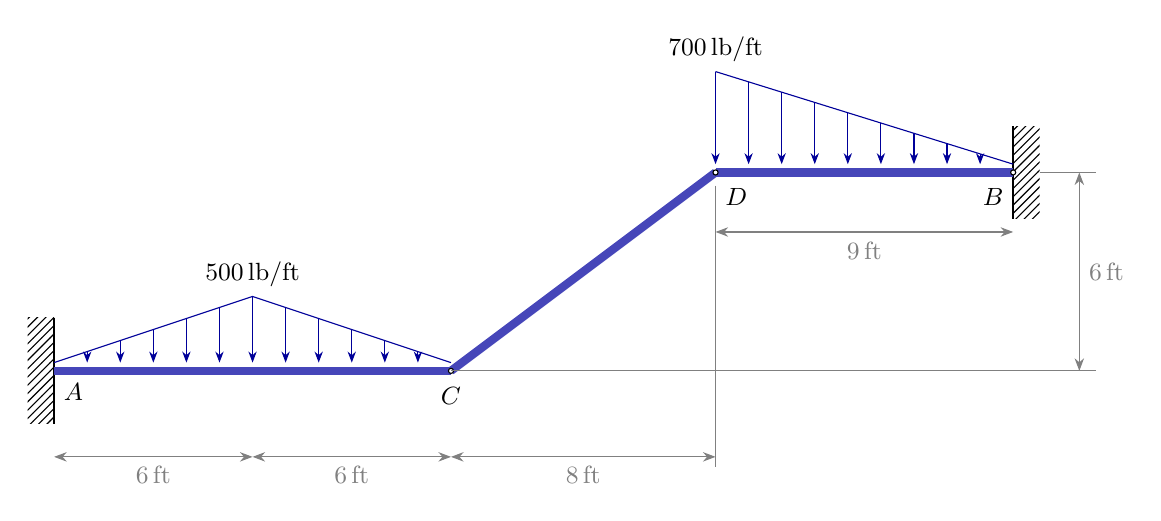
\begin{tikzpicture}[scale=0.42]
% walls
\fill[pattern=north east lines] (-0.8,-1.6) rectangle (0,1.6); \draw[thick] (0,-1.6) -- (0,1.6);
\fill[pattern=north east lines] (29,4.6) rectangle (29.8,7.4); \draw[thick] (29,4.6) -- (29,7.4);
% members
\draw[mem] (0,0) -- (12,0); \draw[mem] (12,0) -- (20,6); \draw[mem] (20,6) -- (29,6);
\pin{12,0} \pin{20,6} \pin{29,6}
% load on AC
\draw[load] (0,0.25) -- (6,2.25) -- (12,0.25);
\foreach \x in {1,...,11} \draw[loadarrow] (\x,{0.25+2*(1-abs(\x-6)/6)}) -- (\x,0.25);
\node[above] at (6,2.25) {\SI{500}{lb/ft}};
% load on DB
\draw[load] (20,9.05) -- (29,6.25);
\foreach \x in {20,...,28} \draw[loadarrow] (\x,{6.25+2.8*(1-(\x-20)/9)}) -- (\x,6.25);
\node[above] at (20,9.05) {\SI{700}{lb/ft}};
% labels
\node[below right] at (0,-0.1) {$A$};
\node[below] at (12,-0.2) {$C$};
\node[below right] at (20,5.8) {$D$};
\node[below left] at (29,5.8) {$B$};
% dims
\draw[dim] (0,-2.6) -- (6,-2.6) node[midway,below]{\SI{6}{ft}};
\draw[dim] (6,-2.6) -- (12,-2.6) node[midway,below]{\SI{6}{ft}};
\draw[dim] (12,-2.6) -- (20,-2.6) node[midway,below]{\SI{8}{ft}};
\draw[thin,gray] (20,5.6) -- (20,-2.9);
\draw[dim] (20,4.2) -- (29,4.2) node[midway,below]{\SI{9}{ft}};
\draw[thin,gray] (12,0) -- (31.5,0);
\draw[dim] (31,0) -- (31,6) node[midway,right]{\SI{6}{ft}};
\draw[thin,gray] (29.8,6) -- (31.5,6);
\end{tikzpicture}

\vspace{0.5cm}

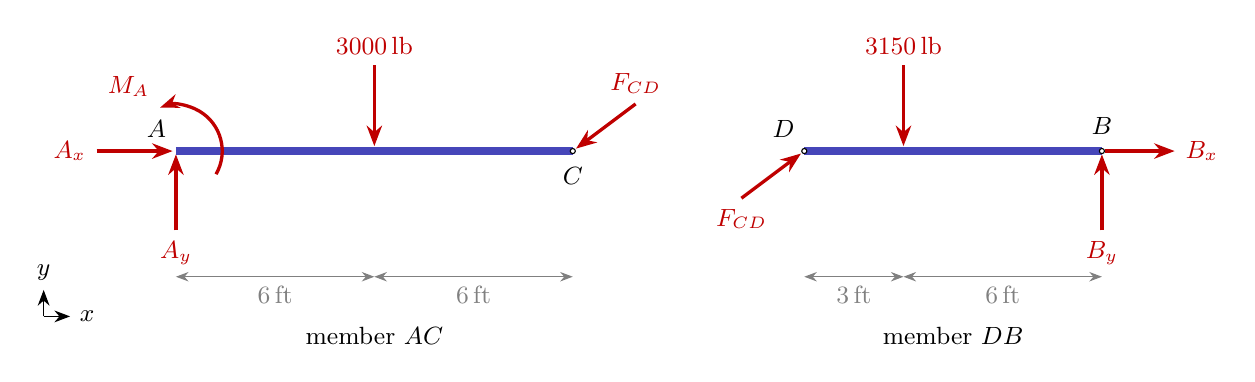
\begin{tikzpicture}[scale=0.42]
% FBD AC
\draw[mem] (0,0) -- (12,0); \pin{12,0}
\node[above left] at (0,0.1) {$A$}; \node[below] at (12,-0.2) {$C$};
\draw[force] (-2.4,0) -- (-0.1,0) node[pos=0,left]{$A_x$};
\draw[force] (0,-2.4) -- (0,-0.1) node[pos=0,below]{$A_y$};
\draw[-{Stealth[length=2.4mm]}, very thick, red!75!black] (-30:1.4) arc (-30:110:1.4) node[above left]{$M_A$};
\draw[force] (6,2.6) -- (6,0.15) node[pos=0,above]{\SI{3000}{lb}};
\draw[force] (13.9,1.425) -- (12.1,0.075) node[pos=0,above]{$F_{CD}$};
\draw[dim] (0,-3.8) -- (6,-3.8) node[midway,below]{\SI{6}{ft}};
\draw[dim] (6,-3.8) -- (12,-3.8) node[midway,below]{\SI{6}{ft}};
\node at (6,-5.6) {member $AC$};
\axes{(-4,-5)}
% FBD DB
\begin{scope}[xshift=19cm]
\draw[mem] (0,0) -- (9,0); \pin{0,0} \pin{9,0}
\node[above left] at (0,0.1) {$D$}; \node[above] at (9,0.2) {$B$};
\draw[force] (-1.9,-1.425) -- (-0.1,-0.075) node[pos=0,below]{$F_{CD}$};
\draw[force] (3,2.6) -- (3,0.15) node[pos=0,above]{\SI{3150}{lb}};
\draw[force] (9.1,0) -- (11.2,0) node[right]{$B_x$};
\draw[force] (9,-2.4) -- (9,-0.1) node[pos=0,below]{$B_y$};
\draw[dim] (0,-3.8) -- (3,-3.8) node[midway,below]{\SI{3}{ft}};
\draw[dim] (3,-3.8) -- (9,-3.8) node[midway,below]{\SI{6}{ft}};
\node at (4.5,-5.6) {member $DB$};
\end{scope}
\end{tikzpicture}
\end{center}

\textbf{Solution:}

$CD$ is a two-force member on a 3-4-5 slope: components $\tfrac45F_{CD}$ horizontal, $\tfrac35F_{CD}$ vertical (compression assumed).

Load resultants:
\[
F_{AC} = \tfrac12(500)(12) = \SI{3000}{lb} \text{ at \SI{6}{ft} from } A, \qquad
F_{DB} = \tfrac12(700)(9) = \SI{3150}{lb} \text{ at \SI{3}{ft} from } D
\]

\textit{Member $DB$:}
\begin{align*}
\textstyle\sum M_B &= (\SI{3150}{lb})(\SI{6}{ft}) - \tfrac35F_{CD}(\SI{9}{ft}) = 0 \;\Rightarrow\; F_{CD} = \SI{3500}{lb}\text{ (C)}\\
\textstyle\sum F_x &= \tfrac45(3500) + B_x = 0 \;\Rightarrow\; B_x = \SI{-2800}{lb}\\
\textstyle\sum F_y &= \tfrac35(3500) - 3150 + B_y = 0 \;\Rightarrow\; B_y = \SI{1050}{lb}
\end{align*}

\textit{Member $AC$} ($CD$ pushes $C$ with $(-2800, -2100)$\,lb):
\begin{align*}
\textstyle\sum F_x &= A_x - 2800 = 0 \;\Rightarrow\; A_x = \SI{2800}{lb}\\
\textstyle\sum F_y &= A_y - 3000 - 2100 = 0 \;\Rightarrow\; A_y = \SI{5100}{lb}\\
\textstyle\sum M_A &= M_A - (3000)(6) - (2100)(12) = 0 \;\Rightarrow\; M_A = \SI{43200}{lb.ft}
\end{align*}

\begin{finalanswer}
$A_x = \SI{2800}{lb}$, \quad $A_y = \SI{5100}{lb}$, \quad $M_A = \SI{43200}{lb.ft}$ (CCW)\\[2pt]
$B_x = \SI{-2800}{lb}$ (left), \quad $B_y = \SI{1050}{lb}$
\end{finalanswer}

% =========================================================
% PROBLEM 3
% =========================================================
\problemhead{3}{A \SI{75}{kg} cylinder hangs from a cable over a \SI{0.3}{m} pulley at the end of $CB$, then runs horizontally back to the wall. Bent member $AB$ is pinned at $A$, runs \SI{2}{m} right and \SI{1.5}{m} up to $B$; the pulley center is \SI{0.5}{m} past $B$. Find the force components at pins $B$ and $C$.}

\textbf{Sketch:}

\begin{center}
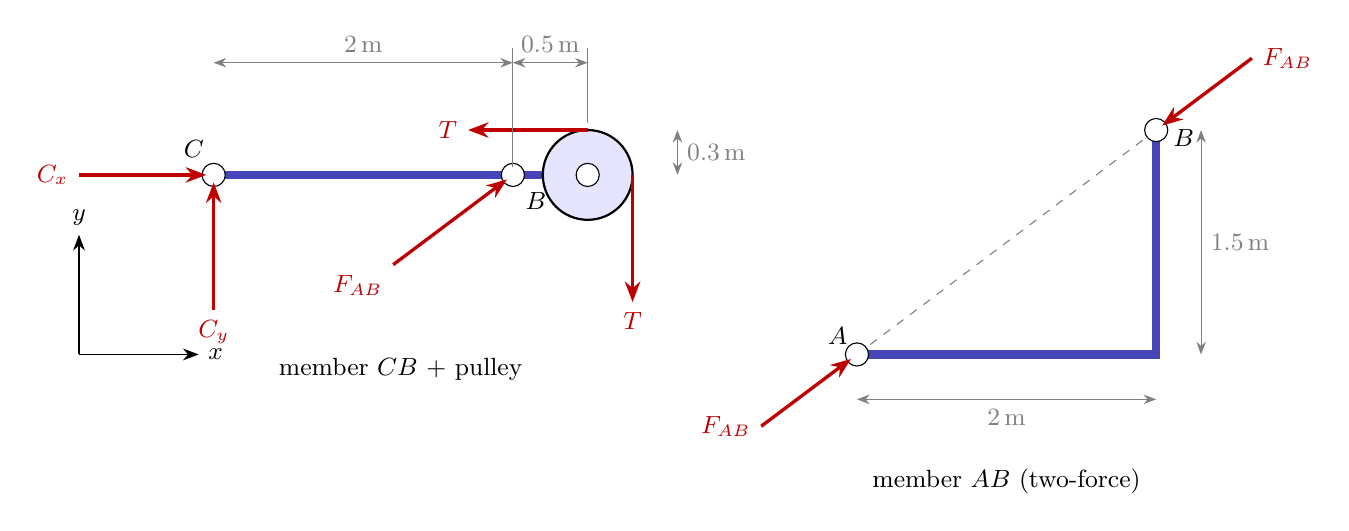
\begin{tikzpicture}[scale=1.9]
% CB + pulley FBD (origin at C)
\draw[mem] (0,0) -- (2.5,0);
\draw[thick,fill=blue!10] (2.5,0) circle (0.3);
\pin{0,0} \pin{2,0} \pin{2.5,0}
\node[above left] at (0,0.05) {$C$};
\node[below right] at (2.02,-0.05) {$B$};
\draw[force] (-0.9,0) -- (-0.05,0) node[pos=0,left]{$C_x$};
\draw[force] (0,-0.9) -- (0,-0.05) node[pos=0,below]{$C_y$};
\draw[force] (2.5,0.3) -- (1.7,0.3) node[left]{$T$};
\draw[force] (2.8,0) -- (2.8,-0.85) node[below]{$T$};
\draw[force] (1.2,-0.6) -- (1.96,-0.03) node[pos=0,below left]{$F_{AB}$};
\draw[dim] (0,0.75) -- (2,0.75) node[midway,above]{\SI{2}{m}};
\draw[dim] (2,0.75) -- (2.5,0.75) node[midway,above]{\SI{0.5}{m}};
\draw[thin,gray] (2,0.05) -- (2,0.85); \draw[thin,gray] (2.5,0.35) -- (2.5,0.85);
\draw[dim] (3.1,0) -- (3.1,0.3) node[midway,right]{\SI{0.3}{m}};
\node at (1.25,-1.3) {member $CB$ + pulley};
\axes{(-0.9,-1.2)}
% AB FBD
\begin{scope}[xshift=4.3cm,yshift=-1.2cm]
\draw[mem] (0,0) -- (2,0) -- (2,1.5);
\draw[dashed,gray] (0,0) -- (2,1.5);
\pin{0,0} \pin{2,1.5}
\node[above left] at (0,0) {$A$}; \node[right] at (2.05,1.45) {$B$};
\draw[force] (2.64,1.98) -- (2.04,1.53) node[pos=0,right]{$F_{AB}$};
\draw[force] (-0.64,-0.48) -- (-0.04,-0.03) node[pos=0,left]{$F_{AB}$};
\draw[dim] (0,-0.3) -- (2,-0.3) node[midway,below]{\SI{2}{m}};
\draw[dim] (2.3,0) -- (2.3,1.5) node[midway,right]{\SI{1.5}{m}};
\node at (1,-0.85) {member $AB$ (two-force)};
\end{scope}
\end{tikzpicture}
\end{center}

\textbf{Solution:}

$T = mg = (75)(9.81) = \SI{735.75}{N}$.

$AB$ is a two-force member along a 3-4-5 line; assume compression, so it acts on $CB$ at $B$ with $(\tfrac45F_{AB}, \tfrac35F_{AB})$.

\textit{Member $CB$:}
\begin{align*}
\textstyle\sum M_C &= \tfrac35F_{AB}(\SI{2}{m}) + T(\SI{0.3}{m}) - T(\SI{2.8}{m}) = 0 \;\Rightarrow\; F_{AB} = \frac{(2.5)(735.75)}{1.2} = \SI{1532.8}{N}\\
B_x &= \tfrac45(1532.8) = \SI{1226}{N}, \qquad B_y = \tfrac35(1532.8) = \SI{919.7}{N}\\
\textstyle\sum F_x &= C_x + 1226 - 735.75 = 0 \;\Rightarrow\; C_x = \SI{-490.5}{N}\\
\textstyle\sum F_y &= C_y + 919.7 - 735.75 = 0 \;\Rightarrow\; C_y = \SI{-183.9}{N}
\end{align*}

\begin{finalanswer}
$B_x = \SI{1230}{N}$, \quad $B_y = \SI{920}{N}$ \quad ($AB$ in compression)\\[2pt]
$C_x = \SI{-491}{N}$, \quad $C_y = \SI{-184}{N}$
\end{finalanswer}

% =========================================================
% PROBLEM 4
% =========================================================
\problemhead{4}{The frame rests on rollers at $A$ and $C$ with \SI{6}{kN} down at $G$. Find the forces in $FD$ and $BD$ and the pin reactions at $C$ on $ABC$ and on $CDE$.}

\textbf{Sketch:}

\begin{center}
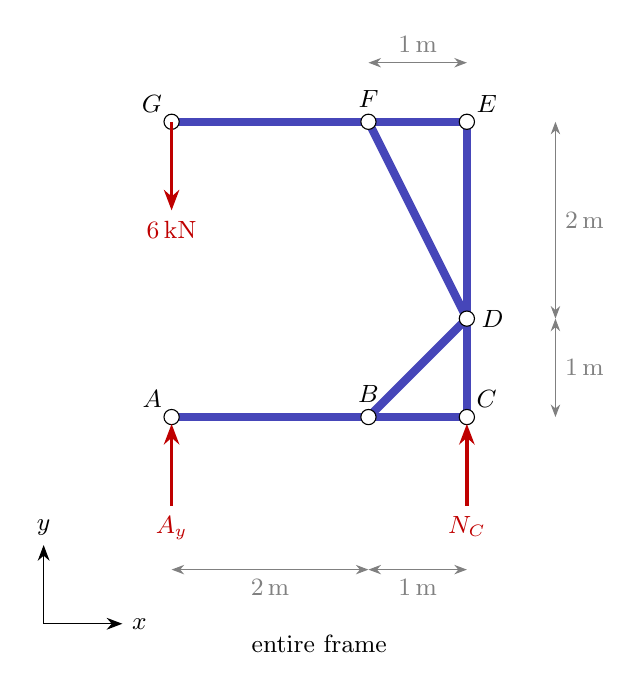
\begin{tikzpicture}[scale=1.25]
\draw[mem] (0,3) -- (3,3); \draw[mem] (3,0) -- (3,3); \draw[mem] (0,0) -- (3,0);
\draw[mem] (2,3) -- (3,1); \draw[mem] (2,0) -- (3,1);
\foreach \p in {{0,3},{2,3},{3,3},{3,1},{2,0},{0,0},{3,0}} {\pin{\p}}
\node[above left] at (0,3) {$G$}; \node[above] at (2,3.05) {$F$}; \node[above right] at (3,3) {$E$};
\node[right] at (3.05,1) {$D$}; \node[above] at (2,0.05) {$B$};
\node[above left] at (0,0) {$A$}; \node[above right] at (3,0) {$C$};
\draw[force] (0,3) -- (0,2.1) node[below]{\SI{6}{kN}};
\draw[force] (0,-0.9) -- (0,-0.07) node[pos=0,below]{$A_y$};
\draw[force] (3,-0.9) -- (3,-0.07) node[pos=0,below]{$N_C$};
\draw[dim] (0,-1.55) -- (2,-1.55) node[midway,below]{\SI{2}{m}};
\draw[dim] (2,-1.55) -- (3,-1.55) node[midway,below]{\SI{1}{m}};
\draw[dim] (2,3.6) -- (3,3.6) node[midway,above]{\SI{1}{m}};
\draw[dim] (3.9,0) -- (3.9,1) node[midway,right]{\SI{1}{m}};
\draw[dim] (3.9,1) -- (3.9,3) node[midway,right]{\SI{2}{m}};
\node at (1.5,-2.3) {entire frame};
\axes{(-1.3,-2.1)}
\end{tikzpicture}

\vspace{0.6cm}

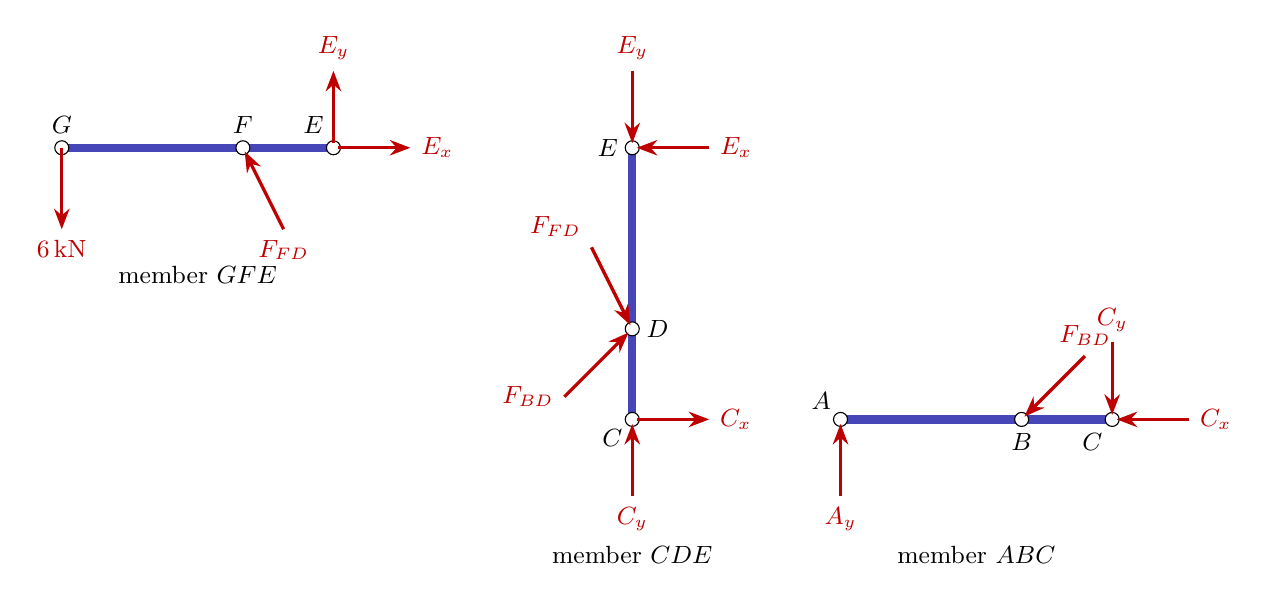
\begin{tikzpicture}[scale=1.15]
% GFE
\draw[mem] (0,3) -- (3,3); \pin{0,3} \pin{2,3} \pin{3,3}
\node[above] at (0,3.05) {$G$}; \node[above] at (2,3.05) {$F$}; \node[above left] at (3,3.05) {$E$};
\draw[force] (0,3) -- (0,2.1) node[below]{\SI{6}{kN}};
\draw[force] (2.45,2.1) -- (2.02,2.96) node[pos=0,below]{$F_{FD}$};
\draw[force] (3.05,3) -- (3.85,3) node[right]{$E_x$};
\draw[force] (3,3.05) -- (3,3.85) node[above]{$E_y$};
\node at (1.5,1.6) {member $GFE$};
% CDE
\begin{scope}[xshift=6.3cm]
\draw[mem] (0,0) -- (0,3); \pin{0,0} \pin{0,1} \pin{0,3}
\node[left] at (-0.05,3) {$E$}; \node[right] at (0.05,1) {$D$}; \node[below left] at (0,0) {$C$};
\draw[force] (0.85,3) -- (0.05,3) node[pos=0,right]{$E_x$};
\draw[force] (0,3.85) -- (0,3.05) node[pos=0,above]{$E_y$};
\draw[force] (-0.45,1.9) -- (-0.02,1.04) node[pos=0,above left]{$F_{FD}$};
\draw[force] (-0.75,0.25) -- (-0.04,0.96) node[pos=0,left]{$F_{BD}$};
\draw[force] (0.05,0) -- (0.85,0) node[right]{$C_x$};
\draw[force] (0,-0.85) -- (0,-0.05) node[pos=0,below]{$C_y$};
\node at (0,-1.5) {member $CDE$};
\end{scope}
% ABC
\begin{scope}[xshift=8.6cm]
\draw[mem] (0,0) -- (3,0); \pin{0,0} \pin{2,0} \pin{3,0}
\node[above left] at (0,0) {$A$}; \node[below] at (2,-0.05) {$B$}; \node[below left] at (3,-0.05) {$C$};
\draw[force] (0,-0.85) -- (0,-0.05) node[pos=0,below]{$A_y$};
\draw[force] (2.7,0.7) -- (2.03,0.03) node[pos=0,above]{$F_{BD}$};
\draw[force] (3.85,0) -- (3.05,0) node[pos=0,right]{$C_x$};
\draw[force] (3,0.85) -- (3,0.05) node[pos=0,above]{$C_y$};
\node at (1.5,-1.5) {member $ABC$};
\end{scope}
\end{tikzpicture}
\end{center}

\textbf{Solution:}

$FD$ (length $\sqrt5$\,m) and $BD$ (length $\sqrt2$\,m) are two-force members, assumed in compression.

\textit{Entire frame:} $\sum M_A = N_C(\SI{3}{m}) = 0 \Rightarrow N_C = 0$, so $A_y = \SI{6}{kN}$.

\textit{Member $GFE$:}
\begin{align*}
\textstyle\sum M_E &= (6)(3) - \tfrac{2}{\sqrt5}F_{FD}(1) = 0 \;\Rightarrow\; F_{FD} = 9\sqrt5 = \SI{20.1}{kN}\text{ (C)}\\
\textstyle\sum F_x &= E_x - \tfrac{1}{\sqrt5}(20.1) = 0 \;\Rightarrow\; E_x = \SI{9}{kN}\\
\textstyle\sum F_y &= E_y + 18 - 6 = 0 \;\Rightarrow\; E_y = \SI{-12}{kN}
\end{align*}

\textit{Member $CDE$} ($(-9, 12)$\,kN at $E$, $(9,-18)$\,kN from $FD$ and $\tfrac{1}{\sqrt2}F_{BD}(1,1)$ from $BD$, both at $D$):
\begin{align*}
\textstyle\sum M_C &= (9)(3) - (9)(1) - \tfrac{1}{\sqrt2}F_{BD}(1) = 0 \;\Rightarrow\; F_{BD} = 18\sqrt2 = \SI{25.5}{kN}\text{ (C)}\\
\textstyle\sum F_x &= -9 + 9 + 18 + C_x = 0 \;\Rightarrow\; C_x = \SI{-18}{kN}\\
\textstyle\sum F_y &= 12 - 18 + 18 + C_y = 0 \;\Rightarrow\; C_y = \SI{-12}{kN}
\end{align*}

\begin{finalanswer}
$F_{BD} = \SI{25.5}{kN}$ (C), \quad $F_{FD} = \SI{20.1}{kN}$ (C)\\[2pt]
Pin $C$ on $CDE$: $C_x = \SI{-18.0}{kN}$, $C_y = \SI{-12.0}{kN}$\\[2pt]
Pin $C$ on $ABC$: $C_x = \SI{18.0}{kN}$, $C_y = \SI{12.0}{kN}$
\end{finalanswer}

% =========================================================
% PROBLEM 5
% =========================================================
\problemhead{5}{A toggle clamp must press on the workpiece at $A$ with \SI{300}{N}. Find the handle force $F$, applied perpendicular to the handle.}

\textbf{Assumptions:} $C$ and $D$ sit \SI{30}{mm} above and below the arm centerline, \SI{235}{mm} from $A$. $B$ is on the centerline, \SI{70}{mm} right of $C$. Link $BE$ is \SI{30}{\degree} from vertical, and the handle is \SI{30}{\degree} above horizontal. As in the textbook solution, the \SI{275}{mm} is measured along the handle from the point directly above $B$ at the level of $C$.

\textbf{Sketch:}

\begin{center}
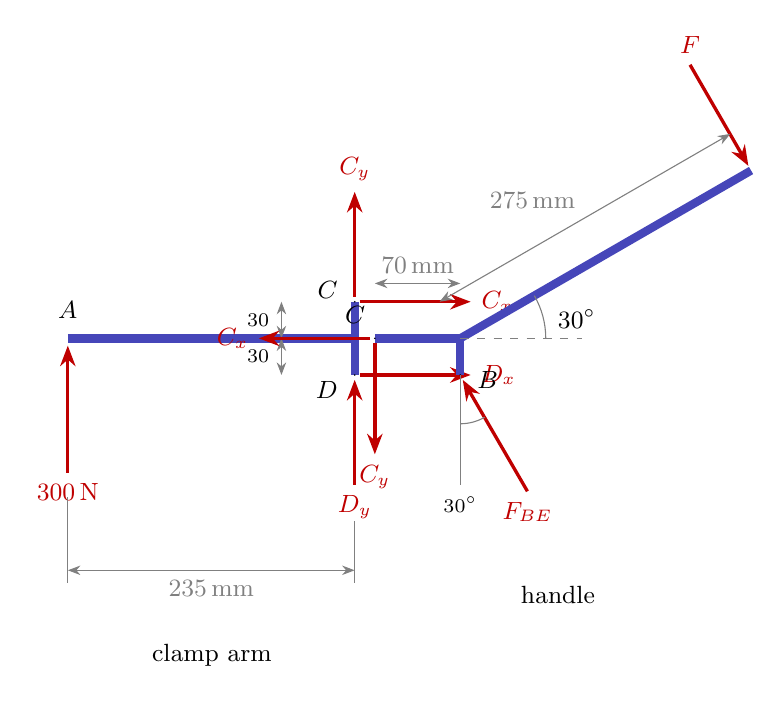
\begin{tikzpicture}[scale=0.0155]
% Arm FBD (origin on centerline at C/D line)
\draw[mem] (-235,0) -- (0,0); \draw[mem] (0,-30) -- (0,30);
\pin{0,30} \pin{0,-30}
\node[left] at (-6,40) {$C$}; \node[left] at (-6,-42) {$D$}; \node[above] at (-235,8) {$A$};
\draw[force] (-235,-110) -- (-235,-6) node[pos=0,below]{\SI{300}{N}};
\draw[force] (4,30) -- (95,30) node[right]{$C_x$};
\draw[force] (0,34) -- (0,120) node[above]{$C_y$};
\draw[force] (4,-30) -- (95,-30) node[right]{$D_x$};
\draw[force] (0,-120) -- (0,-34) node[pos=0,below]{$D_y$};
\draw[dim] (-235,-190) -- (0,-190) node[midway,below]{\SI{235}{mm}};
\draw[thin,gray] (0,-150) -- (0,-200); \draw[thin,gray] (-235,-130) -- (-235,-200);
\draw[dim] (-60,0) -- (-60,30); \draw[dim] (-60,0) -- (-60,-30);
\node[left] at (-62,15) {\scriptsize 30}; \node[left] at (-62,-15) {\scriptsize 30};
\node at (-117,-260) {clamp arm};
% Handle FBD (origin at C)
\begin{scope}[xshift=470]
\draw[mem] (0,0) -- (70,0) -- (70,-30); \draw[mem] (70,0) -- (308.2,137.5);
\pin{0,0} \pin{70,-30}
\node[above left] at (0,4) {$C$}; \node[right] at (76,-34) {$B$};
\draw[dashed,gray] (70,0) -- (170,0);
\draw[gray] (140,0) arc (0:30:70); \node[right] at (142,16) {$30^\circ$};
\draw[force] (-4,0) -- (-95,0) node[left]{$C_x$};
\draw[force] (0,-4) -- (0,-95) node[below]{$C_y$};
\draw[force] (258.2,224.1) -- (306,141.3) node[pos=0,above]{$F$};
\draw[force] (125,-125.3) -- (72,-34) node[pos=0,below]{$F_{BE}$};
\draw[gray] (70,-30) -- (70,-120); \draw[gray] (90,-64.6) arc (-60:-90:40);
\node[below] at (70,-122) {\scriptsize $30^\circ$};
\draw[dim] (0,45) -- (70,45) node[midway,above]{\SI{70}{mm}};
\draw[dim] ($(70,0)+(-17,30)$) -- ($(308.2,137.5)+(-17,30)$) node[midway,above left]{\SI{275}{mm}};
\node at (150,-210) {handle};
\end{scope}
\end{tikzpicture}
\end{center}

\textbf{Solution:}

\textit{Clamp arm,} $\sum M_D$:
\[
\textstyle\sum M_D = -(300)(235) - C_x(60) = 0 \;\Rightarrow\; C_x = \SI{-1175}{N}
\]
The arm pushes the handle at $C$ with \SI{1175}{N} to the right.

\textit{Handle.} $BE$ (two-force, compression) acts on $B$ along $(-\sin30^\circ, \cos30^\circ)$; $F$ acts along $(\sin30^\circ, -\cos30^\circ)$.
\[
\textstyle\sum F_x = 1175 - F_{BE}\sin30^\circ + F\sin30^\circ = 0 \;\Rightarrow\; F_{BE} = 2350 + F
\]
$\sum M_C$, with $B = (70,-30)$\,mm and $F$ at $(70 + 275\cos30^\circ,\ 275\sin30^\circ) = (308.2,\ 137.5)$\,mm:
\begin{align*}
\textstyle\sum M_C &= F_{BE}\big[(70)\cos30^\circ - (30)\sin30^\circ\big] - F\big[(308.2)\cos30^\circ + (137.5)\sin30^\circ\big] = 0\\
&= 45.62\,(2350 + F) - 335.7\,F = 0\\
F &= \frac{(45.62)(2350)}{335.7 - 45.62} = \SI{369.6}{N}
\end{align*}
$F_{BE} = \SI{2720}{N}$ (C).

\begin{finalanswer}
$F = \SI{370}{N}$
\end{finalanswer}

% =========================================================
% PROBLEM 6
% =========================================================
\problemhead{6}{Crank $AB$ (\SI{8}{in}) and link $BC$ (\SI{12}{in}) drive piston $C$ between smooth vertical walls. The spring ($k = \SI{15}{lb/in}$) is unstretched at $\theta = 0^\circ$. Find the couple $M$ on $AB$ for equilibrium at $\theta = 30^\circ$.}

\textbf{Sketch:}

\begin{center}
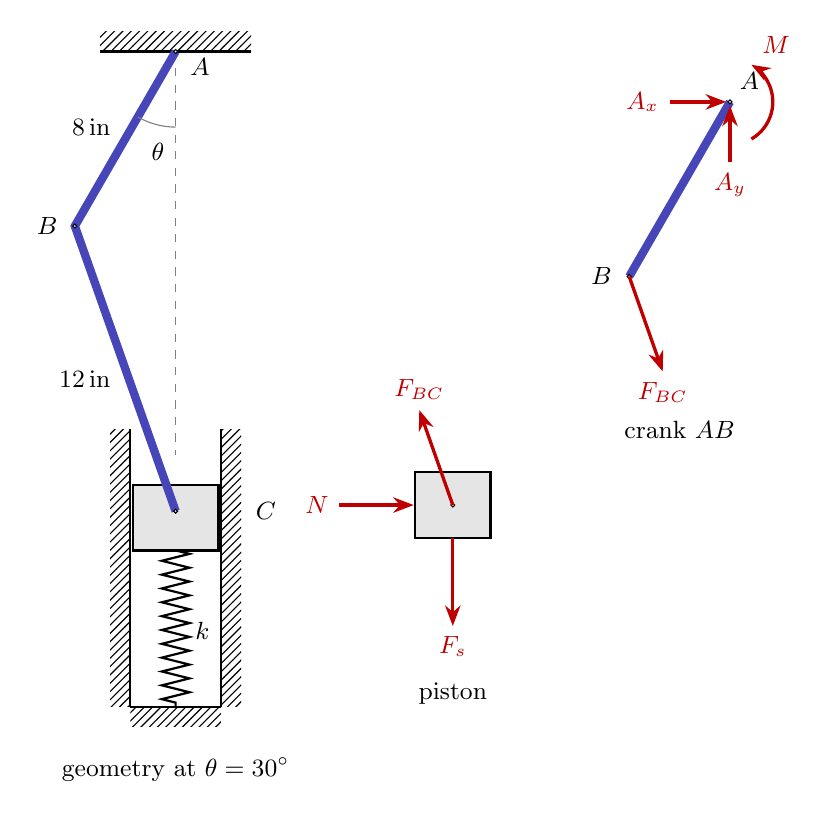
\begin{tikzpicture}[scale=0.32]
% Geometry
\fill[pattern=north east lines] (-3,0) rectangle (3,0.8); \draw[thick] (-3,0) -- (3,0);
\draw[dashed,gray] (0,0) -- (0,-16);
\fill[pattern=north east lines] (-2.6,-15) rectangle (-1.8,-26); \draw[thick] (-1.8,-15) -- (-1.8,-26);
\fill[pattern=north east lines] (1.8,-15) rectangle (2.6,-26); \draw[thick] (1.8,-15) -- (1.8,-26);
\draw[thick,fill=gray!20] (-1.7,-19.8) rectangle (1.7,-17.2);
\draw[thick,decorate,decoration={zigzag,segment length=5,amplitude=5}] (0,-19.8) -- (0,-26);
\fill[pattern=north east lines] (-1.8,-26.8) rectangle (1.8,-26); \draw[thick] (-1.8,-26) -- (1.8,-26);
\draw[mem] (0,0) -- (-4,-6.928) -- (0,-18.242);
\pin{0,0} \pin{-4,-6.928} \pin{0,-18.242}
\node[right] at (0.2,-0.6) {$A$}; \node[left] at (-4.3,-6.928) {$B$}; \node[right] at (2.8,-18.242) {$C$};
\draw[gray] (0,-3) arc (-90:-120:3); \node at (-0.7,-4) {$\theta$};
\node[left] at (-2.2,-3.0) {\SI{8}{in}}; \node[left] at (-2.2,-13) {\SI{12}{in}};
\node[right] at (0.4,-23) {$k$};
\node at (0,-28.5) {geometry at $\theta = 30^\circ$};
% Piston FBD
\begin{scope}[xshift=11cm,yshift=-18cm]
\draw[thick,fill=gray!20] (-1.5,-1.3) rectangle (1.5,1.3); \pin{0,0}
\draw[force] (0,0) -- (-1.33,3.77) node[above]{$F_{BC}$};
\draw[force] (0,-1.3) -- (0,-4.8) node[below]{$F_s$};
\draw[force] (-4.5,0) -- (-1.55,0) node[pos=0,left]{$N$};
\node at (0,-7.5) {piston};
\end{scope}
% Crank FBD
\begin{scope}[xshift=22cm,yshift=-2cm]
\draw[mem] (0,0) -- (-4,-6.928); \pin{0,0} \pin{-4,-6.928}
\node[above right] at (0,0.1) {$A$}; \node[left] at (-4.3,-6.928) {$B$};
\draw[force] (-2.4,0) -- (-0.15,0) node[pos=0,left]{$A_x$};
\draw[force] (0,-2.4) -- (0,-0.15) node[pos=0,below]{$A_y$};
\draw[-{Stealth[length=2.4mm]}, very thick, red!75!black] (-60:1.7) arc (-60:60:1.7) node[above right]{$M$};
\draw[force] (-4,-6.928) -- (-2.67,-10.70) node[below]{$F_{BC}$};
\node at (-2,-13) {crank $AB$};
\end{scope}
\end{tikzpicture}
\end{center}

\textbf{Solution:}

\textit{Geometry} (origin at $A$). $B = (-8\sin30^\circ, -8\cos30^\circ) = (-4, -6.928)$\,in. $BC$ spans \SI{4}{in} horizontally and $\sqrt{12^2 - 4^2} = \SI{11.314}{in}$ vertically, so $C$ is \SI{18.242}{in} below $A$ (\SI{20}{in} at $\theta = 0^\circ$):
\[
\delta = 20 - 18.242 = \SI{1.758}{in}, \qquad F_s = k\delta = (15)(1.758) = \SI{26.37}{lb}
\]

\textit{Piston} (walls push horizontally only):
\[
\textstyle\sum F_y = F_{BC}\left(\tfrac{11.314}{12}\right) - 26.37 = 0 \;\Rightarrow\; F_{BC} = \SI{27.97}{lb}
\]

\textit{Crank $AB$.} $BC$ (tension) pulls $B$ with $F_{BC}\left(\tfrac{4}{12}, -\tfrac{11.314}{12}\right) = (9.32,\ -26.37)$\,lb:
\begin{align*}
\textstyle\sum M_A &= M + \big[(-4)(-26.37) - (-6.928)(9.32)\big] = M + 170.1 = 0\\
M &= \SI{-170.1}{lb.in}
\end{align*}

\begin{finalanswer}
$M = \SI{170}{lb.in}$ (clockwise)
\end{finalanswer}

% =========================================================
% PROBLEM 7
% =========================================================
\problemhead{7}{The ``A'' frame is held by smooth collars at $A$ and $E$ and a pin at $G$. $B$, $C$, $D$, $F$ are ball-and-sockets, with $F$ midway between $B$ and $D$. The pin at $G$ fails at \SI{800}{N}. Find the largest $P$ (load $-P\mathbf k$ at $C$) and the force components $BD$ exerts on $ABC$ and $EDC$.}

\textbf{Assumptions:} The collars slide on a shaft along $x$, so they resist only $y$ and $z$ forces. The pin at $G$ resists force only. Coordinates (m):
\[
A(0.3,0,0),\ E(-0.3,0,0),\ G(0,0,-0.6),\ C(0,1.2,0),\ B(0.15,0.6,0),\ D(-0.15,0.6,0),\ F(0,0.6,0)
\]

\textbf{Sketch:}

\begin{center}
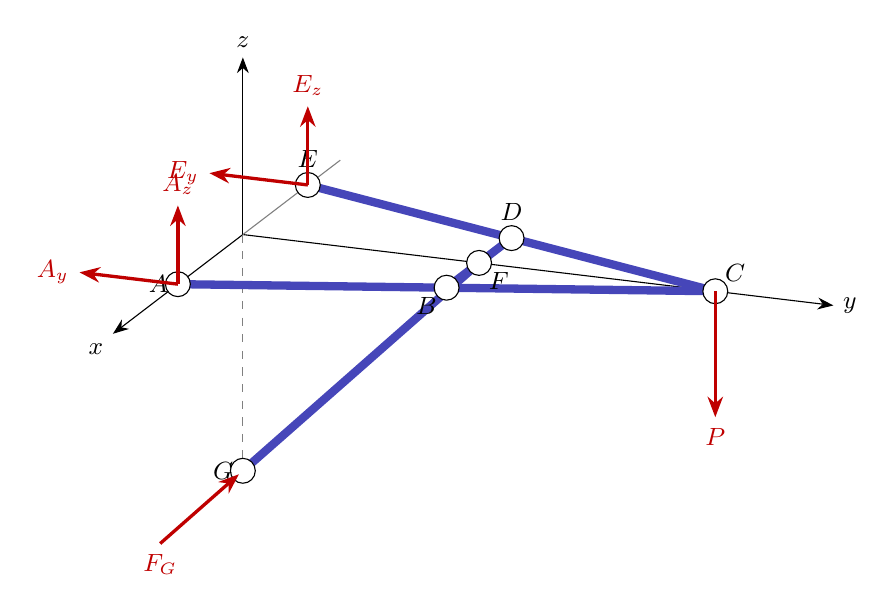
\begin{tikzpicture}[x={(-0.55cm,-0.42cm)}, y={(1cm,-0.12cm)}, z={(0cm,1cm)}, scale=5]
% axes
\draw[axis] (0,0,0) -- (0.6,0,0) node[below left]{$x$};
\draw[axis] (0,0,0) -- (0,1.5,0) node[right]{$y$};
\draw[axis] (0,0,0) -- (0,0,0.45) node[above]{$z$};
\draw[thin,gray] (-0.45,0,0) -- (0,0,0);
\draw[thin,gray,dashed] (0,0,0) -- (0,0,-0.6);
% members
\draw[mem] (0.3,0,0) -- (0,1.2,0);
\draw[mem] (-0.3,0,0) -- (0,1.2,0);
\draw[mem] (0.15,0.6,0) -- (-0.15,0.6,0);
\draw[mem] (0,0,-0.6) -- (0,0.6,0);
\foreach \p in {{0.3,0,0},{-0.3,0,0},{0,0,-0.6},{0,1.2,0},{0.15,0.6,0},{-0.15,0.6,0},{0,0.6,0}} {\fill[white] (\p) circle (0.9pt); \draw (\p) circle (0.9pt);}
\node[left] at (0.3,0,0) {$A$}; \node[above] at (-0.3,0,0.02) {$E$};
\node[left] at (0,0,-0.6) {$G$}; \node[above right] at (0,1.2,0) {$C$};
\node[below left] at (0.15,0.6,0) {$B$}; \node[above] at (-0.15,0.6,0.02) {$D$};
\node[below right] at (0,0.6,0) {$F$};
% loads and reactions
\draw[force] (0,1.2,0) -- (0,1.2,-0.32) node[below]{$P$};
\draw[force] (0,-0.21,-0.81) -- (0,-0.01,-0.61) node[pos=0,below]{$F_G$};
\draw[force] (0.3,0,0) -- (0.3,0,0.2) node[above]{$A_z$};
\draw[force] (0.3,0,0) -- (0.3,-0.25,0) node[left]{$A_y$};
\draw[force] (-0.3,0,0) -- (-0.3,0,0.2) node[above]{$E_z$};
\draw[force] (-0.3,0,0) -- (-0.3,-0.25,0) node[left]{$E_y$};
\end{tikzpicture}
\end{center}

\textbf{Solution:}

\textit{Member $FG$} (two-force, compression): $\vec{GF} = (0, 0.6, 0.6)$\,m, so the force on the frame at $G$ is $F_G\,\mathbf u_{GF}$ with $\mathbf u_{GF} = (0, \tfrac{1}{\sqrt2}, \tfrac{1}{\sqrt2})$.

\textit{Entire frame,} $\sum M_x$ ($M_x = yF_z - zF_y$):
\[
\textstyle\sum M_x = (1.2)(-P) - (-0.6)\dfrac{F_G}{\sqrt2} = 0 \;\Rightarrow\; P = \dfrac{0.6}{1.2\sqrt2}F_G = 0.3536\,F_G
\]
With $F_G = \SI{800}{N}$: $P_{\max} = (0.3536)(800) = \SI{282.8}{N}$.

\textit{Member $BD$.} $FG$ loads $BD$ at $F$ with $(0, 565.7, 565.7)$\,N. Let $(B_x, B_y, B_z)$ be the force of $BD$ on $ABC$; by symmetry $BD$ feels $(-B_x, -B_y, -B_z)$ at $B$ and $(B_x, -B_y, -B_z)$ at $D$:
\[
\textstyle\sum F_y = 565.7 - 2B_y = 0 \;\Rightarrow\; B_y = \SI{282.8}{N}, \qquad
\sum F_z = 565.7 - 2B_z = 0 \;\Rightarrow\; B_z = \SI{282.8}{N}
\]
$B_x$ drops out of $BD$'s equations, so it comes from $ABC$.

\textit{Member $ABC$.} Each leg carries $P/2 = \SI{141.4}{N}$ at $C$, and the legs interact there only along $x$. Forces: $(0, A_y, A_z)$ at $A$, $(B_x, 282.8, 282.8)$ at $B$, $(C_x, 0, -141.4)$ at $C$; $\vec r_{AB} = (-0.15, 0.6, 0)$, $\vec r_{AC} = (-0.3, 1.2, 0)$:
\begin{align*}
\textstyle\sum F_x &= B_x + C_x = 0 \;\Rightarrow\; C_x = -B_x\\
\textstyle\sum M_{A,z} &= \big[(-0.15)(282.8) - (0.6)B_x\big] - (1.2)C_x = -42.43 + 0.6B_x = 0 \;\Rightarrow\; B_x = \SI{70.7}{N}
\end{align*}

\begin{finalanswer}
$P_{\max} = \SI{283}{N}$\\[2pt]
$BD$ on $ABC$ (at $B$): $(\SI{70.7}{N},\ \SI{283}{N},\ \SI{283}{N})$\\[2pt]
$BD$ on $EDC$ (at $D$): $(\SI{-70.7}{N},\ \SI{283}{N},\ \SI{283}{N})$
\end{finalanswer}

\end{document}